\section{Theorie}
\label{sec:Theorie}
Mittels der Kernspinresonanz
können ein Teile der magnetische Momente von Atomkernen
in einer Probe
durch Anlegen eines
äußern Magnetfeldes
gezielt verändet werden und somit
eine makroskopische Magnetisierung der Probe
erzeugen.
Durch die Kernspinresonaz ist es möglich
Aussagen zur Molekulstruktur wie z.B. chemischen Bindungen
zu machen.
Desweiteren können auch mikroskopische
Relaxationsprozesse innerhalb der Probe
durch anlegen eines
äußern magnetischen Wechselfeldes
untersucht
werden.


% Einleitung
% kurze zusammen fassung kernspinresonaz
\subsection{Kernspinresonaz}
Zunächst soll die Magnetisierung einer Probe
in einem Magnetfeld $\vec{B}=B_0\vec{e}_z$,
die sich im thermischen Gleichgewicht befindet, betrachtet werden.
Durch den Zeeman-Effekt
spalten sich die Kernpinzustände mit
Spinquantenzahl $I$ in
 $2I+1$ äquidistante Unterniveaus auf.
 Die Unterniveaus werden mittels
 der Orientierungsquantenzahl $m$
$(-I \leq m \leq I)$ unterschieden und
benachbarte Niveaus besitzen die Energiedifferenz
\begin{align*}
  \Delta E =\gamma B_0 \hbar.
\end{align*}
Die Besetzung im thermischen Gleichgewicht
bei der Temperatur $T$ erfolgt nach der
Bolzmann-Verteilung. Es folgt demnach
für das Besetzungsverhältnis zweier benachbarter Niveaus
\begin{align}
  \frac{N(m)}{N(m-1)} &= \exp\left(-\frac{\gamma B_0 \hbar }{k_B T}\right).
\intertext{Durch die ungeleiche Besetzung
ergibt sich eine Kernspinpolarisation}
\langle I_z \rangle &= \frac{\sum_{m=-I}^{m=I}\hbar m \exp\left(-\frac{m\gamma B_0 \hbar}{k_B T} \right) }{\sum_{m=-I}^{m=I}\exp\left(-\frac{m\gamma B_0 \hbar}{k_B T}\right)}. \label{eqn:I_z}
\end{align}

Werden nur Protonen betrachtet, ergibt
sich, da $I=\tfrac{1}{2}$
eine Aufspaltung, die in der
Abbildung \ref{fig:Proton} dargestellt ist.

\begin{figure}
 \centering
 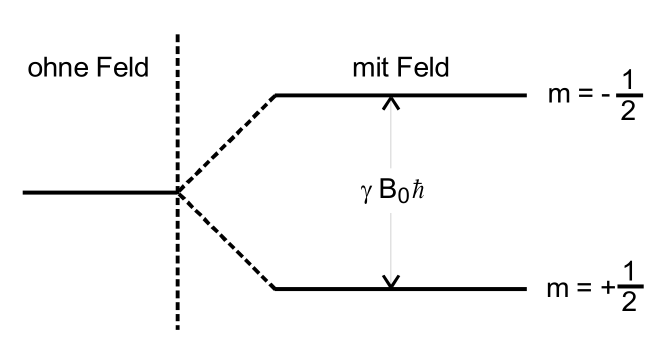
\includegraphics[width=0.5\textwidth]{Zeeman.PNG}
 \caption{Aufspaltung der Energieniveaus im Magnetfeld $B_0$ für $I=\tfrac{1}{2}$.}
 \label{fig:Proton}
\end{figure}
Für Zimmertemperatur und Magnetfelder
der größenordnung $\SI{1}{\tesla}$
gilt $m\gamma B_0 \hbar \ll k_BT$.
Die Kernspinpolarisation für Proton
vereinfacht sich
durch die Näherung zu
\begin{align}
\langle I_z\rangle_P= -\frac{\hbar^2}{4}\frac{\gamma B_0}{k_B T}.
\end{align}
Für die Gleichgewichtsmagnetie
...




\subsection{Larmor-Präzession}
\label{subsec:zielsetzung}

% formeln
\begin{align}
% ddiffusionskonstante
M_Y(t) = M_0\exp\left(-\frac{t}{T_2}\right)
\symup{e}^(-\frac{D\gamma^2 G^2 t^3}{12} \label{}
\end{align}

\subsection{Messmethoden}
\paragraph{Spin-Echo-Methode}
\paragraph{Carr-Pucell-Methode}
\paragraph{Meiboom-Gill-Methode}
\subsection{Einfluss der Diffusion auf Relaxationsverfahren}


\cite{sample}
